\documentclass[a4paper,11pt]{jsarticle}


% 数式
\usepackage{amsmath,amsfonts,amssymb}
\usepackage{bm}
% 画像
\usepackage[dvipdfmx]{graphicx}
\usepackage[dvipdfmx]{color}
\usepackage{siunitx}
\usepackage{wrapfig}
\usepackage{cases}
\usepackage{dcolumn}
\makeatletter
\newcommand{\figcaption}[1]{\def\@captype{figure}\caption{#1}}
\newcommand{\tblcaption}[1]{\def\@captype{table}\caption{#1}}
\makeatother

\usepackage{listings,jvlisting}
\lstset{
basicstyle={\ttfamily},
identifierstyle={\small},
commentstyle={\smallitshape},
keywordstyle={\small\bfseries},
ndkeywordstyle={\small},
stringstyle={\small\ttfamily},
frame={tb},
breaklines=true,
columns=[l]{fullflexible},
numbers=left,
xrightmargin=0zw,
xleftmargin=3zw,
numberstyle={\scriptsize},
stepnumber=1,
numbersep=1zw,
lineskip=-0.5ex
}

\begin{document}

\title{回転軸が円周上を自由に動く剛体2重振り子について}
\author{平林広}
\date{\today}
\maketitle

\begin{figure}[h]
  \centering
  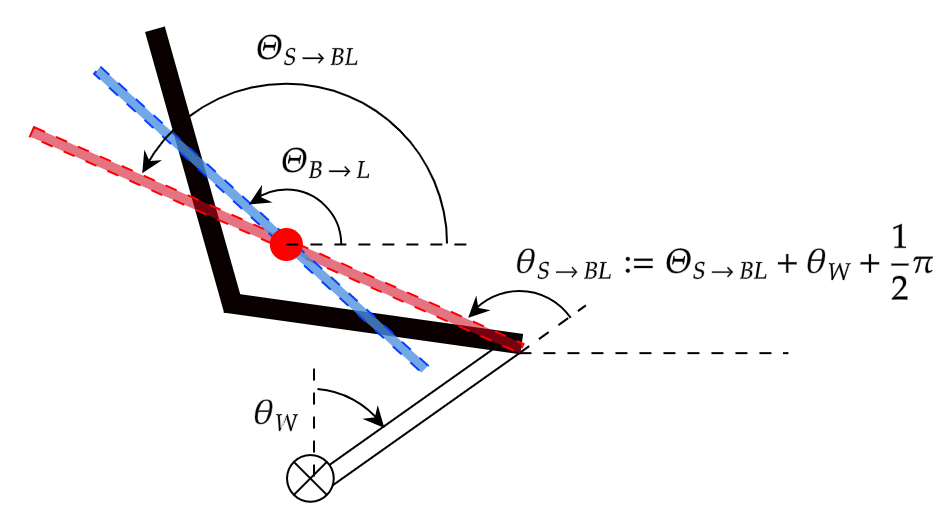
\includegraphics[width = 0.9\textwidth]{conf.png}
  \caption{設定}
  \label{conf.png}
\end{figure}
上肢が全身の質量に対して十分に軽いとし、
上肢の質量と慣性モーメントを$0$とするモデルを考える。
股関節角度が時間変化する場合を考える。

運動方程式は
別PDF「回転軸が円周上を自由に動く剛体単振り子について」を基にする。
変更点は
\begin{gather*}
  \ddot{L} \neq 0
  \\
  \dot{I} \neq 0
  \\
  \dot{I_G} \neq 0
\end{gather*}
であることである。
よって運動方程式は以下の形に変更される。
\begin{align}
  ML\Omega^2 - M\ddot{L}
  =& M(g+a_{PB})\sin\Theta 
  &+& Mr_{arm}\ddot{\theta}_W\sin\theta 
  &-& Mr_{arm}\dot{\theta}_W{}^2\cos\theta 
  \notag
  \\
  &&&&&- F_S\cos\theta
  \label{eq:PB:L_start}
  \\
  I\dot\Omega + \dot{I}\Omega
  =& -M(g+a_{PB}) \cdot L\cos\Theta
  &-& Mr_{arm}\ddot{\theta}_W \cdot L \cos\theta
  &-& Mr_{arm}\dot{\theta}_W{}^2 \cdot L \sin\theta
  &
  \label{eq:PB:I_start}
  \\
  I_G\dot\Omega + \dot{I_G}\Omega
  =& 
  &&&& F_S \cdot L \sin\theta
  \label{eq:PB:IG_start}
\end{align}
ただし
\begin{gather*}
  0\cdot a_{PB} = -k_{PB}y_{PB} + F_S\sin\Theta_W
\end{gather*}
により、$F_S$は既知とし、
$\Theta$として$\Theta_{S\rightarrow BL}, \Theta_{B\rightarrow L}$のどちらを、
$\theta$として$\theta_{S\rightarrow BL}, \theta_{B\rightarrow L}$のどちらを
採用するかは後で述べる。

式 \ref{eq:PB:IG_start}から
\begin{gather}
  \dot{\Omega} = 
  \left.\frac{1}{I_G}\middle(
    F_S \cdot L\sin\theta
    -\dot{I_G}\Omega
  \right)
  \label{eq:Omega}
\end{gather}
を導いておく。

式 \ref{eq:PB:L_start}に$L\cos\theta$、
式 \ref{eq:PB:I_start}に$\sin\theta$をかけて、
$Mr_{Arm}\ddot{\theta}_W$の項を消す。
\begin{gather}
  \left\{
  \begin{aligned}  
    ML^2\Omega^2 - M\ddot{L} \cdot L
    =& M(g+a_{PB})\sin\Theta L\cos\theta
    &+& Mr_{arm}\ddot{\theta}_W\sin\theta L\cos\theta
    &-& Mr_{arm}\dot{\theta}_W{}^2\cos^2\theta \cdot L
    \\
    &&&&&- F_S\cos^2\theta \cdot L
    \\
    I\dot\Omega \sin\theta + \dot{I}\Omega \sin\theta
    =& -M(g+a_{PB}) \cdot L\cos\Theta \sin\theta
    &-& Mr_{arm}\ddot{\theta}_W \cdot L \cos\theta \sin\theta
    &-& Mr_{arm}\dot{\theta}_W{}^2 \cdot L \sin^2\theta
  \end{aligned}
  \right.
  \notag
  \\
  \quad \notag
  \\
  \begin{aligned}
    \Rightarrow
    ML^2\Omega^2 - M\ddot{L}L + I\dot\Omega \sin\theta + \dot{I}\Omega \sin\theta
    =& M(g+a_{PB}) L(\sin\Theta \cos\theta - \cos\Theta \sin\theta)
    \\
    &\quad - Mr_{Arm}L(\cos^2\theta + \sin^2\theta)
    \\
    &\quad - F_S\cos^2\theta \cdot L
  \end{aligned}
  \notag
  \\
  \Rightarrow
  ML^2\Omega^2 - M\ddot{L}L + I\dot\Omega \sin\theta + \dot{I}\Omega \sin\theta
  =
  M(g+a_{PB}) L\sin(\Theta - \theta) - Mr_{Arm}\dot{\theta}_W{}^2L - F_S\cos^2\theta \cdot L
  \notag
\end{gather}
この式から$a_{PB}$を導く。
\begin{align}
  \begin{aligned}
    M(g+a_{PB}) L\sin(\Theta - \theta)
    =&
    ML^2\Omega^2 - M\ddot{L}L + I\dot\Omega \sin\theta + \dot{I}\Omega \sin\theta
    \\
    &\quad + Mr_{Arm}\dot{\theta}_W{}^2L + F_S\cos^2\theta \cdot L
  \end{aligned}
\end{align}
ここで式 \ref{eq:Omega}により
\begin{align}
  \begin{aligned}
    M(g+a_{PB}) L\sin(\Theta - \theta)
    =&
    ML^2\Omega^2 - M\ddot{L}L 
    + \dot{I}\Omega \sin\theta 
    \\
    &\quad + I\sin\theta
    \left.\frac{1}{I_G}\middle(
      F_S \cdot L\sin\theta
      -\dot{I_G}\Omega
    \right)
    \\
    &\quad + Mr_{Arm}\dot{\theta}_W{}^2L + F_S\cos^2\theta \cdot L
  \end{aligned}
  \\
  \begin{aligned}
    \Rightarrow
    M(g+a_{PB}) L\sin(\Theta - \theta)
    =&
    ML^2\Omega^2 - M\ddot{L}L
    + Mr_{Arm}\dot{\theta}_W{}^2L 
    \\
    &\quad
    + \left(
      \dot{I} + \frac{I\dot{I}_G}{I_G}
    \right)
    \Omega\sin\theta
    \\
    &\quad
    + F_S L\left(
      \cos^2\theta + \frac{I}{I_G}\sin^2\theta
    \right)
  \end{aligned}
\end{align}

\end{document}